
\begin{multicols*}{2}

\section{Hunter}

\subsection*{Healing Hands}

\subsection*{Sacred Immolation}

\subsection*{Extra Attack}

Starting at 5th level, you can attack twice, instead of once, whenever you take the Attack action on your turn.

\subsection*{Aura of Courage}

\begin{Figure}
\centering
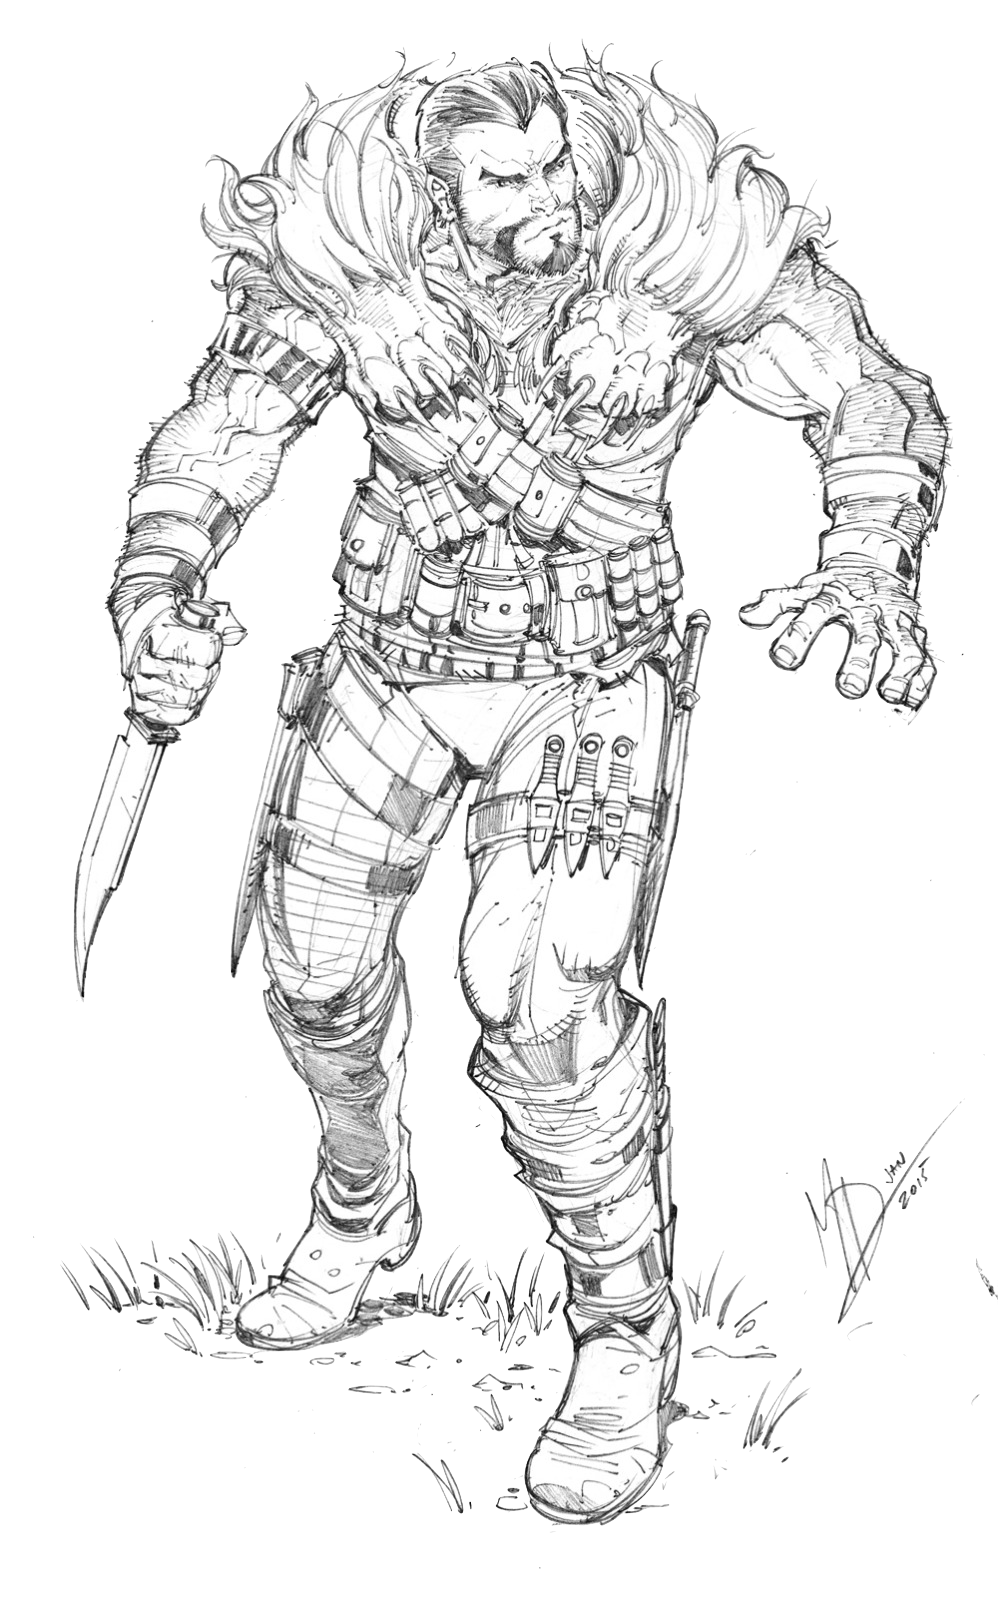
\includegraphics[width=\textwidth]{img/rogue.png}
\end{Figure}
    
\end{multicols*}


\clearpage

\begin{table}[ht!]
\begin{small}
\rowcolors{2}{}{commentgreen}
\begin{center}
\begin{tabular}{ll}
\multicolumn{2}{l}{\parbox[l][0.6cm][c]{15cm}{\textbf{Hunter Cunning Actions}}} 
\\
\hline 
\textbf{Name} & \parbox[l][0.6cm][c]{15cm}{\textbf{Description}}
\\ 
Rain of Arrows & \parbox[l][2cm][c]{15cm}{
As a reaction, you can spend one cunning point to make an attack of opportunity against any creature entering a space 15 feet away from you provided that you are holding a \hl{ranged} weapon.  If you hit, you add the cunning die to the attack's damage roll. Additionally, any feats or benefits applied only to melee weapons apply to your attack.
}
\\ 
Giant Killer & \parbox[l][1.8cm][c]{15cm}{
When a Large or larger creature within 5 feet of you hits or misses you with an attack, you can use a cunning point to spend your reaction to attack that creature immediately after its attack, provided that you can see the creature.  If you hit, you add the cunning die to the attack's damage roll.
}
\\ 
Fast Hands & \parbox[l][1.8cm][c]{15cm}{
You can spend one cunning point and use your bonus action to make a Dexterity (Sleight of Hand) check, open a lock, or take the Use an Object action.
}
\\
Slow Fall & \parbox[l][1.2cm][c]{15cm}{
You can use your reaction when you fall to spend one cunning point and reduce any falling damage you take by an amount equal to five times your cunning die.
}
\\
Augmenting Concoction & \parbox[l][2cm][c]{15cm}{
You can use your bonus action and drink a special potion 
that is toxic to any creature other than you. On you, 
the concotion makes you stronger. Until the end of your next turn, add your cunning die as extra damage to your attack rolls.
}
\\
\hline
\end{tabular}
\end{center}
\end{small}
\end{table} 

    